\subsubsection{\textit{Feature selection} - Unión de \textit{datasets} y filtro de variables}\label{feature-selection}

El \textit{dataset} original \cite{divvy} está divido en años y cada año en múltiples partes. Por lo tanto, la primera tarea de todas ha sido la unión de cada una de estas partes en un único fichero. El formato de archivo ofrecido por \textit{Divvy} es en un CSV como es normal, y por ello se ha usado principalmente la función \verb|read_csv| de pandas que convierte un CSV a un \verb|DataFrame|. Por otro lado, cada parte tenía su propia nomenclatura de columnas por lo que ha sido necesario crear una única nomenclatura para poder trabajar con un único fichero y por ello han sido renombradas algunas columnas. Una vez realizado el renombrado de columnas, el \verb|DataFrame| será anexionado a otro que contendrá todos los datos y que será el que se usará para los siguientes pasos.

\begin{displayquote}
"Un \verb|DataFrame| es una estructura de datos etiquetada en 2 dimensiones con columnas de tipos potencialmente diferentes. Se puede pensar en ello como una hoja de cálculo o una tabla SQL. Generalmente es el objeto más comúnmente usado en la librería de \textit{pandas}." \cite{pandas}
\end{displayquote}

Un ejemplo de \verb|DataFrame| que se ha visto con anterioridad podría ser la tabla \ref{tab:houses}. Para poder inicializar un \verb|DataFrame| se puede realizar desde un diccionario de Python, donde cada clave sea el \verb|string| que identifica a la columna y cada valor sea un vector con la misma cantidad de valores que filas quiere que se tenga. Otra forma de inicializar un \verb|DataFrame| es mediante el uso de funciones como \verb|read_csv()|, \verb|read_h5()| o \verb|read_pickle()|.
\newline

El código usado es algo parecido a lo que se muestra a continuación:

\begin{minted}[fontsize=\footnotesize]{python}
import pandas as pd

# Path to the csv files
csv_filenames = ["trips-2014-Q1", "trips-2014-Q2-Q3", 
                 "trips-2014-Q4", "trips-2015-Q1-Q2",
                 # ...
                 "trips-2019-Q3-Q4"]
csv_paths = [f"/path/to/{file}.csv" for file in csv_filenames]

# This will be the final DataFrame
df = pd.DataFrame()

# For every CSV do
for path in csv_paths:
    
    # CSV to DataFrame
    df_temp = pd.read_csv(path)
    
    # Parse date as datetime which is always first column
    df_temp[cols[0]] = pd.to_datetime(
        df_temp[cols[0]], 
        format='%Y-%m-%d %H:%M:%S',
        infer_datetime_format=True)
    
    # Rename the columns depending on their
    # current names with a external function
    df_temp = rename_columns(df_temp)
    
    # Merge the DataFrames
    df = pd.concat([df, df_temp], join='outer')

# ...
\end{minted}

Una vez obtenido la variable \verb|df| con todos los viajes, se necesita realizar un filtro de las columnas. En este punto, el \verb|DataFrame| contine 12 valores asociados a cada viaje.

\begin{minted}[fontsize=\footnotesize]{python}
df.columns

'''
Index(['trip_id', 'start_time', 'end_time', 'bikeid', 
       'tripduration', 'from_station_id', 
       'from_station_name', 'to_station_id',
       'to_station_name', 'usertype', 'gender',
       'birthyear'],
      dtype='object')
'''
\end{minted}

De este \verb|DataFrame| solo se seleccionan dos:

\begin{itemize}
    \item \textit{start\_time}: Este dato es necesario porque se quiere predecir el uso de bicicletas a partir de una información temporal. Este valor, dado en segundos usando el formato "Tiempo Unix" \cite{unix_time}, nos permite identificar en qué fecha y hora se inició el viaje. Gracias a ello, se pueden identificar distintos patrones, ya que estos varían durante la época del año. No existen los mismos patrones durante el invierno que durante el verano o incluso, no es lo mismo las 2 de la madrugada que las 2 de la tarde.
    \item \textit{from\_station\_id}: Los modelos que se van a construir predecirán el número de viajes que se inician en cada estación de Chicago de forma independiente. Este valor por tanto, será usado para calcular el número de viajes iniciados en un intervalo en cada estación.
\end{itemize}

El resto de atributos también son útiles para otro tipos de problemas como por ejemplo predecir el destino más probable en función de la estación donde se inicia el viaje, u obtener que conexiones son las más transitadas. Sin embargo, está fuera de los objetivos que se han planteado para este trabajo por lo que solo se usarán las columnas previamente mencionadas.
\newline
 
El dataset resultante por tanto, es el mismo dataset original pero con solo las columnas \textit{start\_time} y \textit{from\_station\_id}. En el código esto es fácil de implementar añadiendo solo la siguientes línea:
\begin{minted}[fontsize=\footnotesize]{python}
# ...
    
# Filter the columns that we need
cols = ["start_time", "from_station_id"]
df = df[cols]

# Save the DataFrame in a CSV
df.to_csv("trips.csv", index=False)
\end{minted}

Se podrían haber usado más columnas que ayudasen a la predicción, sin embargo, por falta de tiempo y porque los resultados obtenidos eran de por sí bastante buenos, no se ha visto la necesidad de añadirlos.
\newline

Gráficamente este módulo realiza lo siguiente:
\begin{figure}[H]
    \centering
    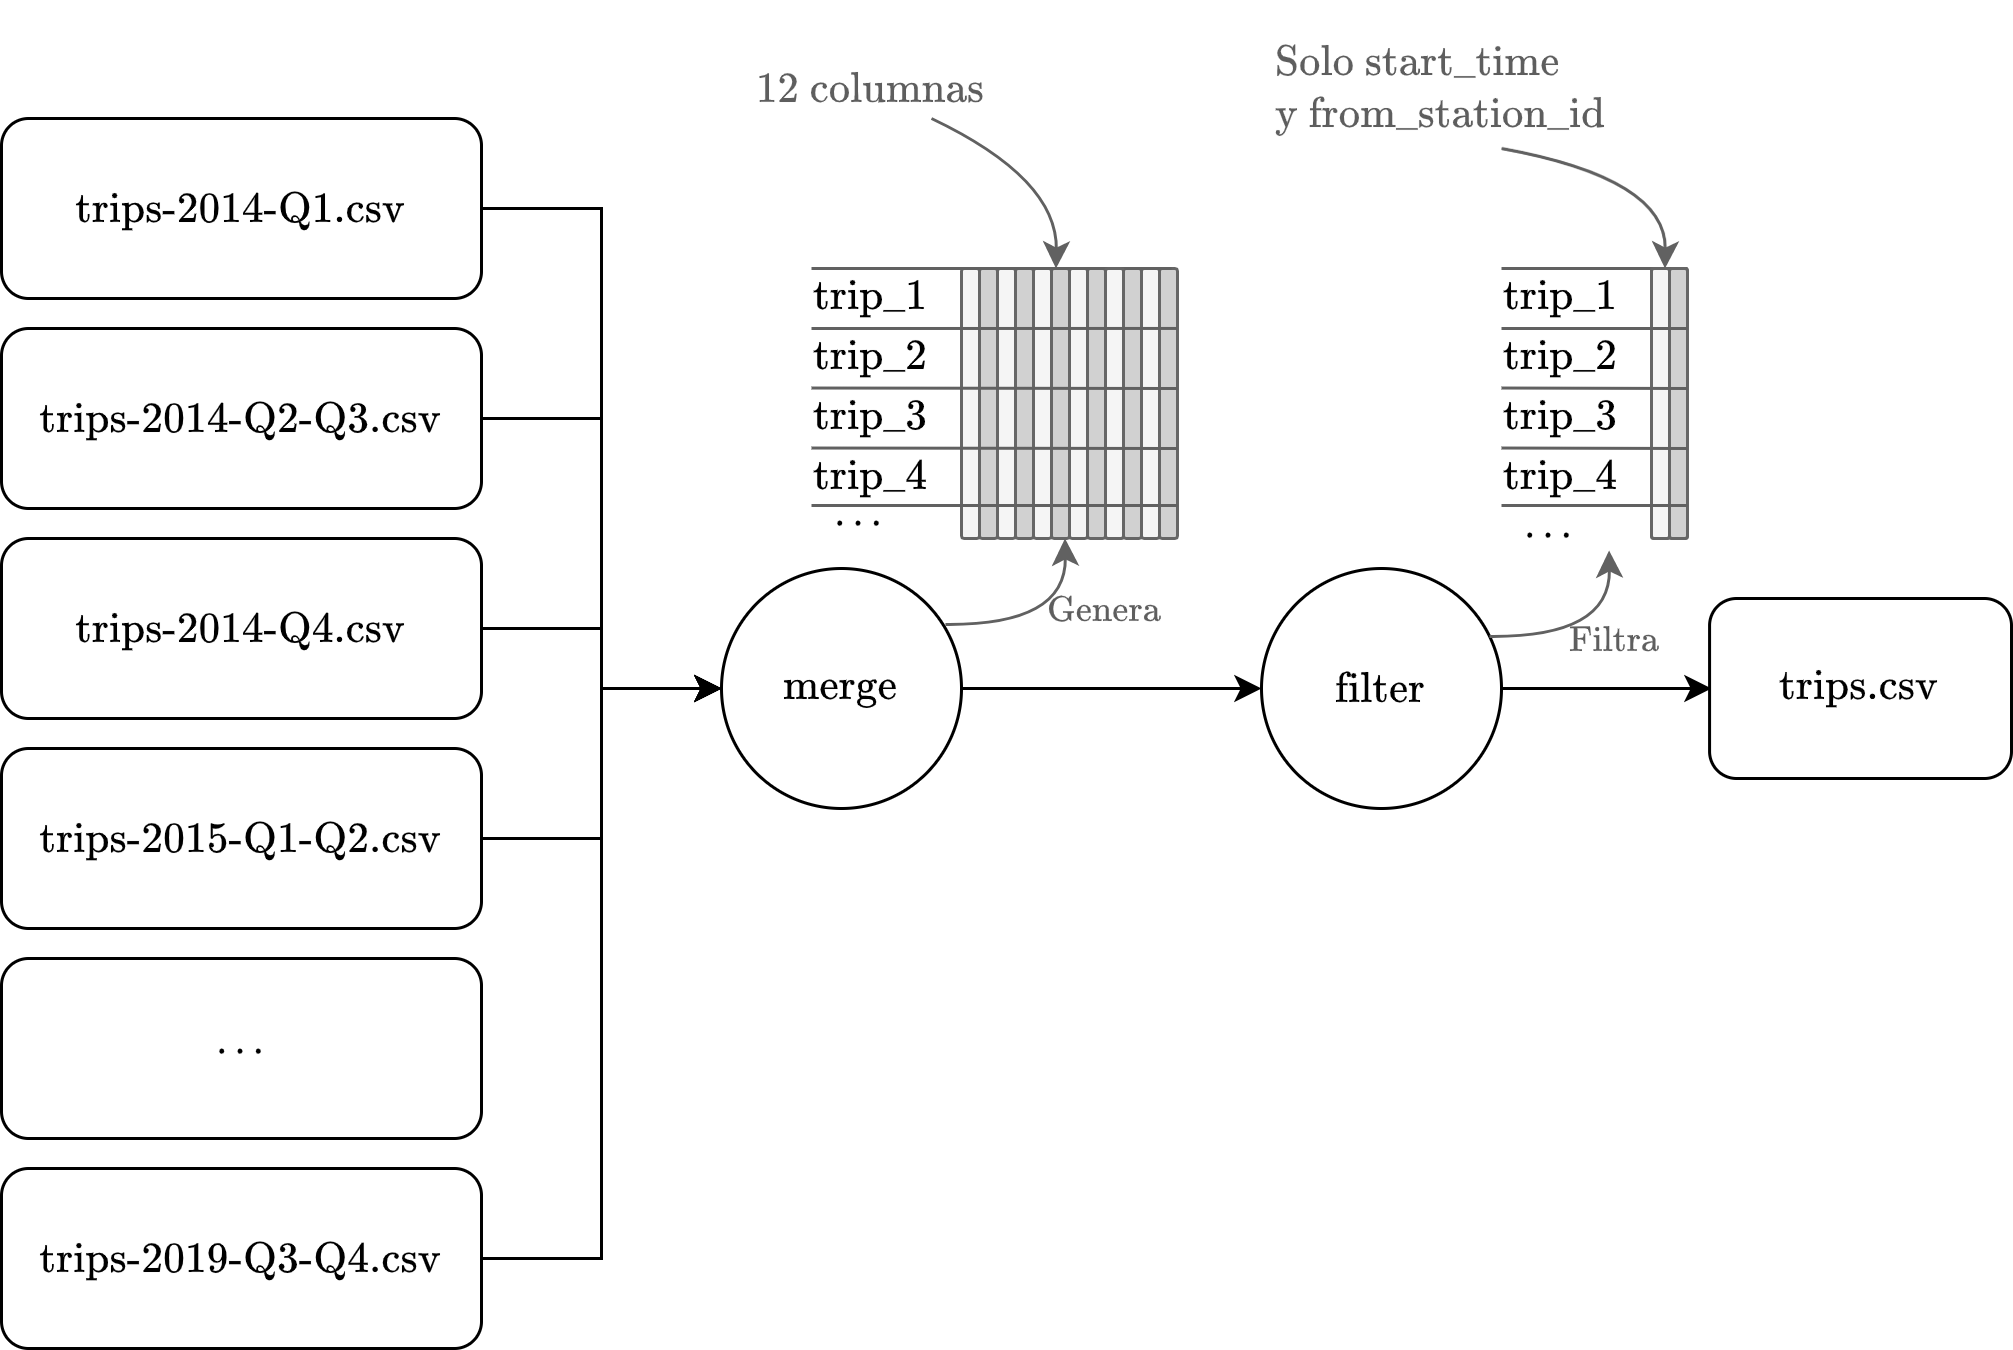
\includegraphics[width=12cm]{images/solution/modules/feature-selection.png}
    \caption{Estructura del módulo \textit{feature-selection}.}
\end{figure}